\subsection{System design}
% metatext & redesignmotivation
In the second iteration the \gls{rs} system were designed to consists of three parts: The \gls{rs} app, the \gls{rs} server, and the \gls{astep} system.
As the \gls{astep} system have evolved small redesigns to the \gls{rs} system design is necessary.

%User management
The \gls{astep} system have the responsibility to create, manage and delete users who exists in the several \gls{astep} apps.
During the development of the user management system, several ideas have been shared which lead to a few different implementation trough the sprint.
The user management system ended up implement user groups.
User groups are implemented to ensure privacy, so only users within the same group can access each other location data.

Every user would need to add every other user, in the \gls{rs} system, in order to access each other data.
This would lead to unnecessary load on the \gls{astep} server as the user base would grow bigger and the API calls would grow exponential.
An example of this is seen on \ref{fig:userbefore} with a group of five users where each arrow represent an API call that allows access to a users data.
This leads to a redesign of the \gls{rs} system as it should be transparent and every user need to have access to every other users data.

\begin{figure}[!h]
	\centering
	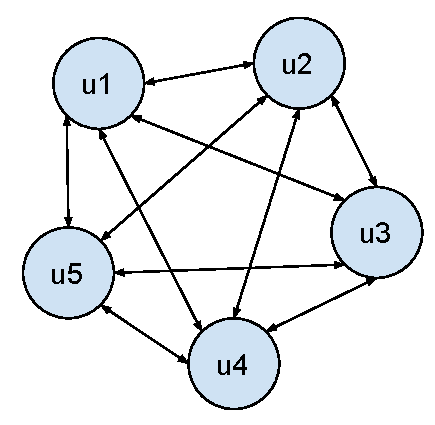
\includegraphics[width=0.35\textwidth]{figures/userbefore.pdf}
	\caption{System design, including all major parts of the solution.}
	\label{fig:userbefore}
\end{figure}

%RSS admin user
In order to allow each user to see every other user, the \gls{rs} server would be set as an administrator user, who would have access to every others users data.
The server will then handle users data that are communicated between the \gls{astep} server, \gls{rs} server. 
This completely removes the need for users to be within a group with every other user and saves a lot of API calls.
This design can be seen on \ref{fig:userafter} where the admin user marked with \"A\" will be used as a middle point who can access every users data and therefore reducing the number API calls.

\begin{figure}[!h]
	\centering
	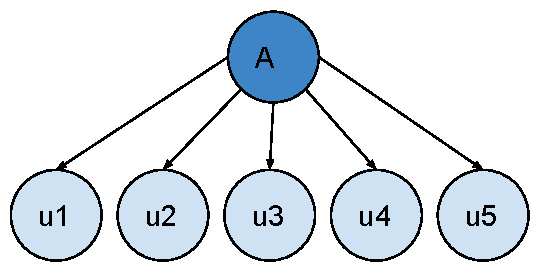
\includegraphics[width=0.35\textwidth]{figures/userafter.pdf}
	\caption{System design, including all major parts of the solution.}
	\label{fig:userafter}
\end{figure}

In the second iteration it were also decided to created a user through the \gls{rs} server, this have been changed to simplify the implementation.
When a user registers in the app an API call will be issued to the \gls{astep} API directly from the app where before this was done through the \gls{rs} server. 
The username and the additional information such as phone number and full name are still transfered to the \gls{rs} server for storing.
